\documentclass[t]{beamer}
\usetheme[deutsch]{KIT}
\setbeamercovered{transparent}
\setbeamertemplate{navigation symbols}{}

\KITfoot{Tutoriumsmaterial von Joachim Priesner, Sebastian Ullrich und Max Wagner \hspace{2.5cm} Basierend auf den Folien von Simon Stroh und Moritz v. Looz}
\usepackage[utf8]{inputenc}
\usepackage{amsmath}
\usepackage{ifthen}
\usepackage{amssymb}
\usepackage{tikz}
\usepackage{ngerman}
\usetikzlibrary{automata}
\usenavigationsymbols


\title{Theoretische Grundlagen der Informatik}
\subtitle{Tutorium}
\author{Moritz von Looz, Simon Stroh}

\institute[ITI]{Institut für Theoretische Informatik}

\TitleImage[height=\titleimageht]{images/tmaschine.png}

\newcommand{\N}{\ensuremath{\mathbb{N}}}
\newcommand{\M}{\ensuremath{\mathcal{M}}}
\newcommand{\classP}{\ensuremath{\mathcal{P}}}
\newcommand{\classNP}{\ensuremath{\mathcal{NP}}}
\newcommand{\pot}{\ensuremath{\mathcal{P}}}
\newcommand{\abs}[1]{\ensuremath{\left\vert #1 \right\vert}}
\newcommand{\menge}[2]{\ensuremath{\left\lbrace #1 \,\middle\vert\, #2 \right\rbrace}}
\newcommand{\ducttape}[1]{\vspace{#1}}
\newcommand{\neglit}[1]{\overline{#1\vphantom{x^a}}}

\newcommand{\invincible}{\setbeamercovered{invisible}} %  "Yesss! I am invincible!!" (Boris Grishenko)
\newcommand{\vincible}{\setbeamercovered{transparent}}

% \@ifundefined{tikzset}{}{\tikzset{initial text=}} % Text "start" bei Startknoten unterdrücken
\tikzstyle{every node}=[thick]
\tikzstyle{every line}=[thick]

\newcommand{\tutnr}[1]{
  \subtitle{Tutorium #1}
	\begin{frame}
		\maketitle
	\end{frame}
}

\newcommand{\uebnr}[1]{
  \subtitle{Anmerkungen zum #1. Übungsblatt}
	\begin{frame}
		\maketitle
	\end{frame}
}

\begin{document}


\subsection{Chomsky-Normalform}
\frame{
\frametitle{Chomsky-Normalform}
CYK wird verwendet zur Lösung des Wortproblems für kontextfreie Sprachen (CH-2).
Um CYK anzuwenden, muss die gegebene Grammatik erst in Chomsky-Normalform gebracht werden. Das ist für jede CH-2 Grammatik möglich.
\
\begin{exampleblock}{Chomsky-Normalform}
Eine CH-2-Grammatik \textit{G} $= \mathcal{(T,V,S,P) }$ ist in Chomsky-Normalform,  wenn jede Produktion aus $\mathcal{P}$ eine der folgenden Formen hat:
\begin{itemize}
\item  $A \rightarrow BC$
\item  $A \rightarrow a$
\end{itemize}
Wobei gilt $A,B,C\in\mathcal{V}$ und $a \in \mathcal{T}$.
Um das leere Wort in der Sprache zu erlauben, lässt sich die Grammatik leicht mit neuem Startsymbol$S'$ ergänzen mit der Regel $$ S' \rightarrow S \mid \varepsilon $$
\end{exampleblock}
}


%\subsection{Umwandlung in Chomsky-Normalform}
\frame{
\frametitle{Umwandlung in Chomsky-Normalform}
\begin{enumerate}
\item Für alle $\textcolor{red}{a} \in \mathcal{T}$ und für alle Produktionen, auf deren rechter Seite $\textcolor{red}{a}$ vorkommt 
(außer für $V  \rightarrow \textcolor{red}{a}$, mit $V \in\mathcal{V}$),
wird jedes Vorkommen von $\textcolor{red}{a}$ durch ein \emph{neues} Nichtterminalsymbol $\textcolor{blue}{A}$ ersetzt
%(und $A$ in die Variablenmenge aufgenommen)
und die Produktion $\textcolor{blue}{A} \rightarrow \textcolor{red}{a}$ wird hinzugefügt.
\end{enumerate}

\begin{exampleblock}{Umwandlungsbeispiel (Schritt 1 von 4)}
\begin{columns}[c]
\begin{column}{0.3\textwidth}
\begin{align*}
\mathcal{S} &\rightarrow XY\\
X &\rightarrow \textcolor{red}{a}X\textcolor{red}{b} \mid Z \mid \varepsilon\\
Y &\rightarrow \textcolor{red}{cc}Y \mid \varepsilon\\
Z &\rightarrow X\\
\end{align*}
\end{column}
%
\
\begin{column}{0.05\textwidth}
$\Rightarrow$
\end{column}
%
\begin{column}{0.3\textwidth}
\begin{align*}
\mathcal{S} &\rightarrow XY\\
X &\rightarrow \textcolor{blue}{A}X\textcolor{blue}{B} \mid Z \mid \varepsilon\\
Y &\rightarrow \textcolor{blue}{CC}Y \mid \varepsilon\\
Z &\rightarrow X\\
\textcolor{blue}{A} &\rightarrow \textcolor{red}{a}\\
\textcolor{blue}{B} &\rightarrow \textcolor{red}{b}\\
\textcolor{blue}{C} &\rightarrow \textcolor{red}{c}\\
\end{align*}
\end{column}
\end{columns}
\end{exampleblock}
}

\begin{frame}
\frametitle{Umwandlung in Chomsky-Normalform}
\begin{enumerate}
\setcounter{enumi}{1}
\item %Die Grammatik $\varepsilon$-frei machen, d. h. $\varepsilon$ darf nur bei $\mathcal{S} \rightarrow \varepsilon$ vorkommen.
In diesem Schritt werden alle Produktionen der Form $\textcolor{red}{V} \rightarrow \textcolor{red}{\varepsilon}$
f"ur $V \in \mathcal{V}, V \not= \mathcal{S}$ entfernt. Dazu müssen diese Produktion aber
vorher \emph{rekursiv} durch ihre ``Vorwegnahme'' mit den anderen Produktionen
``verschmolzen'' werden, es wird also für jede Produktion mit einem der obigen $V$
auf der rechten Seite eine \textcolor{blue}{neue Produktion} ohne dieses $V$ hinzugefügt.
\end{enumerate}

\begin{exampleblock}{Umwandlungsbeispiel (Schritt 2 von 4)}
\begin{columns}[c]
\begin{column}{0.3\textwidth}
\begin{align*}
\mathcal{S} &\rightarrow XY\\
\textcolor{red}{X} &\rightarrow AXB \mid Z \mid \textcolor{red}{\varepsilon}\\
\textcolor{red}{Y} &\rightarrow CCY \mid \textcolor{red}{\varepsilon}\\
Z &\rightarrow X\\
A &\rightarrow a\\
B &\rightarrow b\\
C &\rightarrow c\\
\end{align*}
\end{column}
%
\
\begin{column}{0.05\textwidth}
$\Rightarrow$
\end{column}
%
\begin{column}{0.3\textwidth}
\begin{align*}
\textcolor{blue}{\mathcal{S}} &\rightarrow XY \mid \textcolor{blue}{X} \mid  \textcolor{blue}{Y} \mid \textcolor{blue}{\sout{\varepsilon}}\\
\textcolor{blue}{X} &\rightarrow AXB \mid \textcolor{blue}{AB} \mid Z \\
\textcolor{blue}{Y} &\rightarrow CCY \mid \textcolor{blue}{CC}\\
Z &\rightarrow X\\
A &\rightarrow a\\
B &\rightarrow b\\
C &\rightarrow c\\
\end{align*}
\end{column}
\end{columns}
\end{exampleblock}
\end{frame}



\frame{
\frametitle{Umwandlung in Chomsky-Normalform}
\begin{enumerate}
\setcounter{enumi}{2}
\item
Für Produktionen mit mehr als zwei
Variablen rechts werden \textcolor{blue}{ \emph{neue} Nichterminale} eingeführt
und dazu \textcolor{blue}{passende Produktionen} hinzugefügt.
\end{enumerate}

\begin{exampleblock}{Umwandlungsbeispiel (Schritt 3 von 4)}
\begin{columns}[c]
\begin{column}{0.3\textwidth}
\begin{align*}
\mathcal{S} &\rightarrow XY \mid X \mid  Y \\
X &\rightarrow \textcolor{red}{AXB} \mid AB \mid Z \\
Y &\rightarrow \textcolor{red}{CCY} \mid CC\\
Z &\rightarrow X\\
A &\rightarrow a\\
B &\rightarrow b\\
C &\rightarrow c\\
\end{align*}
\end{column}
%
\
\begin{column}{0.05\textwidth}
$\Rightarrow$
\end{column}
%
\begin{column}{0.3\textwidth}
\begin{align*}
\mathcal{S} &\rightarrow XY \mid X \mid  Y\\
X &\rightarrow \textcolor{blue}{FB} \mid AB \mid Z \\
Y &\rightarrow \textcolor{blue}{GY} \mid CC\\
Z &\rightarrow X\\
\textcolor{blue}{F} &\rightarrow \textcolor{blue}{AX}\\
\textcolor{blue}{G} &\rightarrow \textcolor{blue}{CC}\\
A &\rightarrow a\\
B &\rightarrow b\\
C &\rightarrow c\\
\end{align*}
\end{column}
\end{columns}
\end{exampleblock}
}

\frame{
\frametitle{Umwandlung in Chomsky-Normalform}
\begin{enumerate}
\setcounter{enumi}{3}
\item
Für Produktionen mit einer Variablen rechts werden Zyklen gesucht, 
für gefundene Zyklen werden alle Vorkommnisse aller Variablen des Zyklus durch einen Repräsentanten ausgetauscht. Danach werden triviale Produktionen entfernt.
\end{enumerate}

\begin{exampleblock}{Umwandlungsbeispiel (Schritt 4a von 4)}
\begin{columns}[c]
\begin{column}{0.3\textwidth}
\begin{align*}
\mathcal{S} &\rightarrow XY \mid X \mid  Y\\
\textcolor{red}{X} &\rightarrow FB \mid AB \mid \textcolor{red}{Z} \\
Y &\rightarrow GY \mid CC\\
\textcolor{red}{Z} &\rightarrow \textcolor{red}{X}\\
F &\rightarrow AX\\
G &\rightarrow CC\\
A &\rightarrow a\\
B &\rightarrow b\\
C &\rightarrow c\\
\end{align*}
\end{column}
%
\
\begin{column}{0.05\textwidth}
$\Rightarrow$
\end{column}
%
\begin{column}{0.3\textwidth}
\begin{align*}
\mathcal{S} &\rightarrow XY \mid X \mid  Y\\
\textcolor{blue}{X} &\rightarrow \textcolor{blue}{FB} \mid AB \mid \sout{\textcolor{blue}{X}} \\
Y &\rightarrow GY \mid CC\\
\sout{\textcolor{blue}{X}} &\rightarrow \sout{\textcolor{blue}{X}}\\
F &\rightarrow AX\\
G &\rightarrow CC\\
A &\rightarrow a\\
B &\rightarrow b\\
C &\rightarrow c\\
\end{align*}
\end{column}
\end{columns}
\end{exampleblock}
}

\frame{
\frametitle{Umwandlung in Chomsky-Normalform}
\begin{enumerate}
\setcounter{enumi}{3}
\item
Sind alle Zyklen beseitigt, werden im letzten Schritt alle Regeln, die rechts eine einzelne Variable haben, durch ``Vorziehen'' der Regeln eliminiert. (Sollte die $\varepsilon$-Produktion fehlen, wird diese nun eingefügt.
\end{enumerate}

\begin{exampleblock}{Umwandlungsbeispiel (Schritt 4b von 4)}
\begin{columns}[c]
\begin{column}{0.3\textwidth}
\begin{align*}
\mathcal{S} &\rightarrow XY \mid \textcolor{red}{X} \mid  \textcolor{red}{Y}\\
X &\rightarrow FB \mid AB \\
Y &\rightarrow GY \mid CC\\
F &\rightarrow AX\\
G &\rightarrow CC\\
A &\rightarrow a\\
B &\rightarrow b\\
C &\rightarrow c\\
\end{align*}
\end{column}
%
\
\begin{column}{0.05\textwidth}
$\Rightarrow$
\end{column}
%
\begin{column}{0.3\textwidth}
\begin{align*}
\mathcal{S} &\rightarrow XY \mid \textcolor{blue}{FB} \mid \textcolor{blue}{AB} \mid \textcolor{blue}{GY} \mid \textcolor{blue}{CC}\\
X &\rightarrow FB \mid AB \\
Y &\rightarrow GY \mid CC\\
F &\rightarrow AX\\
G &\rightarrow CC\\
A &\rightarrow a\\
B &\rightarrow b\\
C &\rightarrow c\\
\end{align*}
\end{column}
\end{columns}
\end{exampleblock}
}

\begin{frame}
Sei $G=(\Sigma,V,S,R)$ die CH-2-Grammatik mit $\Sigma = \{a,b\}$, $V=\{A,B,C,D,E,S\}$ und der folgenden Regelmenge $R$:
\begin{eqnarray*}
S & \rightarrow & A \;|\; aAa  \;|\; bBb  \;|\; \varepsilon \\
A & \rightarrow & C \;|\; a \\
B & \rightarrow & C \;|\; b \\
C & \rightarrow & CDE \;|\; \varepsilon \\
D & \rightarrow & A \;|\; B \;|\; ab \\
E & \rightarrow & S
\end{eqnarray*}
Bestimme eine Grammatik $G'$ für $L(G)$ in Chomsky-Normalform.
\end{frame}

\frame{
\frametitle{CYK Überblick}
CYK ist ein Algorithmus, um das Wortproblem in CH-2 zu lösen. Um den Algorithmus anzuwenden, muss eine Grammatik in Chomsky-Normalform vorliegen.\\
Grundidee zur Überprüfungen eines Wortes der Länge $n$:
\begin{itemize}
\item Wir betrachen $V_{i,j} = $ Menge der Nichtterminale, aus denen das Teilwort der Position $i$ bis $j$ abgeleitet werden kann
\item Die Lösung ob $V_{i,j}$ ableitbar ist, lässt sich entscheiden durch Betrachten aller möglichen $V_{i,k}$ und $V_{k+1,j}$
\item $V_{i,i}$ sind trivial
\item Bottom-up lässt sich dadurch $V_{1,n}$ berechnen
\item Ist $S \in V_{i,n}$, so lässt sich das Wort ableiten.
\end{itemize}
}

\frame{
\frametitle{CYK}
Gegeben sei die Grammatik \textit{G} $= \mathcal{(T,V,S,P) }$  mit den folgenden Produktionen aus $\mathcal{P}$:
\begin{align*}
\mathcal{S} &\rightarrow XY \mid FB \mid AB \mid  GY\mid CC \mid \lambda\\
X &\rightarrow FB \mid AB \\
Y &\rightarrow GY \mid CC\\
F &\rightarrow AX\\
G &\rightarrow CC\\
A &\rightarrow a\\
B &\rightarrow b\\
C &\rightarrow c\\
\end{align*}
Ist das Wort $abcccc$ in der Sprache $\mathcal{L}(\textit{G})$?
}
\section{11. Tutoriumsvorschlag}
% Pumping Lemma für Kontextfreie Sprachen
\subsection{Pumping Lemma für kontextfreie Sprachen}
\begin{frame}
\frametitle{Pumping-Lemma für kontextfreie Sprachen}
\begin{exampleblock}{Lemma}
Für jede kontextfreie Srache $L$ gibt es eine Konstante $n \in \mathbb{N}$,
so dass sich jedes Wort $z \in L$ mit $|z| \geq n$ so als
$$ z = uvwxy $$
schreiben lässt, dass
\begin{itemize}
\item $|vx| \geq 1$,
\item $|vwx| \leq n$ und
\item für alle $i \geq 0$ das Wort $uv^iwx^iy \in L$ ist.
\end{itemize}
\end{exampleblock}
\end{frame}

\subsection{Ogdens Lemma}
\begin{frame}
\frametitle{Ogdens Lemma für kontextfreie Sprachen}
\begin{exampleblock}{Lemma}
Für jede kontextfreie Sprache $L$
gibt es eine Konstante $n \in \mathbb{N}$ so dass für jedes Wort $z \in L$ mit $|z| \geq n$ gilt:\\
Wenn wir in $z$ mindestens $n$ Buchstaben markieren, so lässt sich $z$ so als $z = uvwxy$ schreiben,
\begin{itemize}
\item dass von den mindestens $n$ markierten Buchstaben
\begin{itemize}
\item mindestens einer zu $vx$ gehört und
\item höchstens $n$ zu $vwx$ gehören und
\end{itemize}
\item für alle $i \geq 0$ das Wort $uv^iwx^iy \in L$ ist.
\end{itemize}
\end{exampleblock}
\end{frame}

\begin{frame}
\frametitle{Beweisidee}
\begin{itemize}
\item Jeder Knoten im Ableitungsbaum (wie wir ihn in CYK sehen) steht für ein Nichtterminalsymbol
\item Ab einer gewissen Höhe des Baumes (bzw. Länge des Wortes) muss ein Nichtterminal im Baum mehrmals in einer Reihe vorkommen
\item Man kann also aus einem Nichtterminalsymbol dasselbe Symbol wieder ableiten
\item Da das Wort durch jede Ableitung (außer zu Terminalsymbolen) länger wird, gibt es eine ``Schleife'' beim Ableiten
\item Diese Schleife kann man also ``pumpen'', also beliebig oft (oder auch gar nicht) durchlaufen
\end{itemize}
\end{frame}

\begin{frame}
\frametitle{Zu Ogden und Pumping ...}
\begin{itemize}
\item Anwendung genau wie ``altes'' Pumping Lemma
\item Wird verwendet, um zu zeigen das eine Sprache nicht kontextfrei ist
\item Dazu: Kontraposition bilden und folgern, dass Sprache nicht kontextfrei
\end{itemize}
\end{frame}

\begin{frame}
\frametitle{Beispiel}
Sei $L = \{a^ib^jc^kd^l | i \neq 0 \Rightarrow j = k = l\}$. Wir zeigen mit Ogdens Lemma, dass $L$ nicht kontextfrei ist.
Für gegebenes $n$ muss das Lemma also für jedes Wort mit $n$ markierten Buchstaben erfüllt sein. Betrachte $z = ab^nc^nd^n \in L$ und markiere $b^n$.
Zu $vx$ muss also immer ein $b$ gehören und in $vwx$ dürfen höchsten $n$ markierte Buchstaben vorkommen. Offensichtlich dürfen in $v$ und $x$ jeweils nur eine Art von Symbol vorkommen. Da aber in $v$ oder $x$ mindestens ein $b$ vorkommen muss, und die Anzahl der $b$ und $c$ und $d$ gleich bleiben muss, ist das Lemma nicht erfüllt. Daher kann $L$ nicht kontextfrei sein.
\end{frame}

\begin{frame}
\frametitle{Aufgabe}
Zeigen Sie, dass folgende Sprachen nicht kontextfrei sind:
\begin{enumerate}
 \item $L=\{a^ib^jc^id^j \mid i,j \geq 1 \}$
 \item $L=\{ww \mid w \text{ ist in }\{a, b\}^* \text{ enthalten.}\}$
\end{enumerate}
\end{frame}

\begin{frame}
\frametitle{Lösungshinweise für Teilaufgabe a}
 Wähle $n$ wie im Pumping-Lemma und $z=a^nb^nc^nd^n$. 
 Zeige dann, dass für jede Zerlegung $z=uvwxy$ gemäß dem Pumping-Lemma $uv^0wx^0y$ nicht in $L$ ist.
\end{frame}
\begin{frame}
 \frametitle{Lösungshinweise für Teilaufgabe b}      
 Teilaufgabe b) kann theoretisch mit dem Pumping-Lemma gezeigt werden (indem man als Wort $a^nb^na^nb^n$ wählt), dazu bekommt man aber eine ziemlich hässliche Fallunterscheidung.
       Einfacher ist es, Ogden's Lemma zu benutzen: 
       \begin{itemize}
        \item Wähle $z=a^nb^na^nb^n$ mit $n$ gemäß Ogden's Lemma.              
        \item Markiere die mittleren beiden Blöcke
        \item Betrachte eine Zerlegung von $z$ gemäß Ogden's Lemma
        \item Dann gehört mindestens einer der Buchstaben von $vx$ zu diesen mittleren Blöcken.
        \end{itemize}
\end{frame}
\begin{frame}
\frametitle{Fallunterscheidung für Teilaufgabe b}
\begin{itemize}
        \item Fall 1: $vx$ enthält mindestens einen Buchstaben aus dem ersten $b$-Block. 
              Dann kann $vx$ keinen Buchstaben aus dem letzten $b$ Block enthalten. 
              Zeige jetzt, dass $uv^0wx^0y$ nicht in $L$ ist: 
              \begin{itemize}
                \item Annahme: $uwy=tt$
                \item $|uwy| \geq 2n$, daraus folgt, dass $t$ mit $b^n$ endet.
                \item Da $vx$ fehlt, gibt es aber keinen zweiten Block der Form $b^n$ in $uwy$, damit kann $t$ nicht nochmal in $uwy$ vorkommen.
                      Also ist $uwy$ nicht in $L$.
              \end{itemize}
        \item Fall 2: $vx$ enthält mindestens einen Buchstaben aus dem zweiten $a$-Block. 
              Dann kann analog zu Fall 1 argumentiert werden. 
       \end{itemize}
\end{frame}

% Greibach-Normalform
\subsection{Greibach-Normalform}
\begin{frame}
\frametitle{Greibach Normalform}
\begin{exampleblock}{Definition}
Eine kontextfreie Grammatik ist in \textbf{Greibach-Normalform}, wenn alle Ableitungsregeln von der Form 
$$ A \rightarrow a\alpha \text{ mit } A \in V\text{,} a\in \Sigma \text{ und } \alpha \in V^*$$
sind.
\end{exampleblock}
\end{frame}

\begin{frame}
\frametitle{Zur Greibach-Normalform}
\begin{itemize}
\item Weitere Normalform für CH-2 Grammatiken, d.h. jede Grammatik kann in Greibach-Normalform gebracht werden
\item Zur Konstruktion von Kellerautomaten aus Grammatiken
\item Es kann stärker, aber äquivalent, verlangt werden, dass auf der rechten Seite höchstens zwei Variablen vorkommen.
\end{itemize}
\end{frame}

\begin{frame}
\frametitle{Umwandlung in Greibach-Normalform}
\begin{exampleblock}{Nebenbemerkung}
Im folgenden stehen Kleinbuchstaben für Terminale, Großbuchstaben für einzelne Nichtterminale und griechische Buchstaben für (eventuell) mehrere Nichtterminale 
\end{exampleblock}
Die Grammatik sei zunächst in Chomsky-Normalform.
\end{frame}

\begin{frame}
\frametitle{Annahmen}
\begin{block}{Annahmen}
\begin{itemize}
 \item Wir gehen davon aus, dass die Grammatik $G$ in Chomsky-Normalform ist, mit $V = \{A_1 ... A_m \}$ und $\Sigma = \{\alpha_1 ... \alpha_n\}$
 \item Folglich sind alle Regeln von der Form $A_i \rightarrow A_jA_k$ oder $A_i \rightarrow \alpha_j$
\end{itemize}
\end{block}
\end{frame}

\begin{frame}
\frametitle{Schritt 1}
Es gebe die Nichtterminale $\{A_0, \ldots, A_N\}$
\begin{enumerate}
\item für alle $i$ in $1, \ldots, N$
\begin{enumerate}
\item für alle $j$ in $1, \ldots, i$
\begin{enumerate}
\item Simuliere alle Regeln für $A_j$ bei Produktionen der Form $A_i \rightarrow A_j\alpha$ mit $j < i$ auf der rechten Seite.
\item für Produktionen der Form $A_i \rightarrow A_i\alpha$ führe eine neue Variable ein (wie: siehe nächste Folie).
\end{enumerate}
\end{enumerate}
\end{enumerate}
\end{frame}

\begin{frame}
\frametitle{$A_i \rightarrow A_i\alpha$}
Für Regeln der Form 
$$A \rightarrow A\alpha_1 \mid \ldots \mid A\alpha_r$$
$$A \rightarrow \beta_1 \mid \ldots \mid \beta_s$$
(wobei $\beta_i$ nicht mit $A$ beginnt) führe ein neues Nichtterminal $\beta$ ein. Ersetze nun die Regeln
$$A \rightarrow A\alpha_1 \mid \ldots \mid A\alpha_r$$
durch
$$A \rightarrow \beta_1B \mid \ldots \mid \beta_sB$$
$$B \rightarrow \alpha_1 \mid \ldots \mid \alpha_r$$
$$B \rightarrow \alpha_1B \mid \ldots \mid \alpha_rB$$
\end{frame}

\begin{frame}
 \frametitle{Schritt 2}
Gehen nun die Produktionen absteigend nach $k$ sortiert durch und simuliere bei alle Regeln mit $A_k \rightarrow A_j\alpha$ die Produktionen für $A_j$ auf der rechten Seite.\\
Da alle Regeln, die mit einem $A_i$ anfangen, der Greibach-Normalform genügen, kann man dieses Verfahren nun bei den neuen Regeln für $B_1,\ldots$ auch anwenden, danach ist die Grammatik in Greibach-Normalform.
\end{frame}

\begin{frame}
\frametitle{Aufgabe zur Greibach-Normalform}
Sei die Grammatik $G$ gegeben durch
\begin{itemize}
 \item $\Sigma = \{0, 1\}$
 \item $V = \{A_1, A_2, A_3\}$
 \item $S = A_1$
 \item $R = \{A_1 \rightarrow A_2A_3, A_2 \rightarrow A_3A_1, A_2 \rightarrow 1, A_3 \rightarrow A_1A_2, A_3 \rightarrow 0\}$
\end{itemize}

Bringen Sie $G$ in Greibach-Normalform.

\textbf{Lösung:} Siehe Skript.
\end{frame}

% Kellerautomaten
\subsection{Kellerautomat}
\begin{frame}
\frametitle{Definition}
Ein (nichtdeterministischer) \textbf{Kellerautomat} (NPDA bzw PDA, Pushdown Automaton) besteht aus $(Q, \Sigma, \Gamma, q_0, Z_0,\delta, F)$, wobei
\begin{itemize}
\item $Q$ endliche Zustandsmenge
\item $\Sigma$ endliches Eingabealphabet
\item $\Gamma$ endliches STACK-Alphabet
\item $q_0 \in Q$ Anfangszustand
\item $Z_0 \in \Gamma$ Initialisierung des STACK
\item $\delta : Q \times ( \Sigma \cup \{\varepsilon\}) \times \Gamma \rightarrow 2^{Q \times \Gamma^*}$
\begin{itemize}
\item $\delta(q, a, Z) \subseteq \{(q,\gamma) : q \in Q, \gamma \in \Gamma^*\}$
\item $\delta(q, \varepsilon, Z) \subseteq \{(q,\gamma) : q \in Q, \gamma \in \Gamma^*\}$
\end{itemize}
\item $F \subseteq Q$ Menge der akzeptierenden Endzustände, $F=\emptyset$ ist möglich.
\end{itemize}
\end{frame}

\begin{frame}
\frametitle{Zu Kellerautomaten}
\begin{itemize}
\item Akzeptieren, wenn \emph{entweder} der Stack leer ist \emph{oder} wenn der Automat in einen akzeptierenden Zustand kommt
\item Sind im allgemeinen nichtdeterministisch
\item Man kann Endzustände auch aus der Definition weglassen und alternativ verlangen, dass der Automat genau bei leerem Keller akzeptiert.
\item Man kann sogar alle Zustände bis auf einen weglassen und alles in die Kellerbelegung kodieren
\end{itemize}
\end{frame}

\begin{frame}
\frametitle{Beispiel}
$M = (Q, \Sigma, \Gamma, q_0, Z_0, \delta, F)$
\begin{itemize}
\item $Q = \{q_0, q_1, q_2\}$, $Z_0 = \{\#\}$
\item $\Sigma = \{a,b\}$
\item $\Gamma = \{\#,X\}$
\item $F = \{q_2\}$
\end{itemize}
\begin{figure}
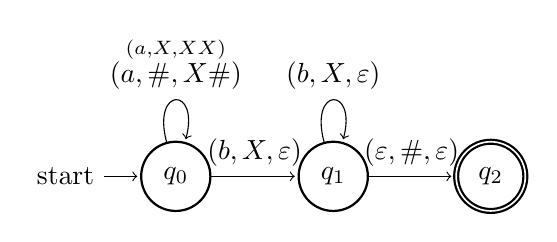
\begin{tikzpicture}[node distance=2cm,shorten >=1pt,auto]
\node[state,initial]   (q_0)                {$q_0$};
\node[state]           (q_1) [right of=q_0] {$q_1$};
\node[state,accepting] (q_2) [right of=q_1] {$q_2$};
\path[->]	(q_0) 	edge 			node {$(b,X,\varepsilon)$}				(q_1)
			edge [loop above]	node {$\stackrel{(a,X,XX)}{(a,\#,X\#)}$}	 	() %stackrel is wrong here.
		(q_1)	edge			node {$(\varepsilon,\#,\varepsilon)$}			(q_2)
			edge [loop above]	node {$(b,X,\varepsilon)$}				();
\end{tikzpicture}
\end{figure}
\end{frame}

\begin{frame}
\frametitle{Aufgaben}
\begin{itemize}
\item Welche Sprache akzeptiert der Beispielautomat der vorigen Folie?
\end{itemize}
\end{frame}

% end of ifthenelse WAY up there
}
%

\section{12. Tutoriumsvorschlag}
%TODO: Beispiel Kellerautomat
\subsection{Kellerautomat aus Greibach-Normalform}
\begin{frame}
 \frametitle{Kellerautomat aus Greibach-Normalform}
 \begin{block}{Erinnerung: Greibach-Normalform}
  Eine kontextfreie Grammatik ist in \textbf{Greibach-Normalform}, wenn alle Ableitungsregeln von der Form   
  \[ A \rightarrow a\alpha \text{ mit } A \in V\text{,} a\in \Sigma \text{ und } \alpha \in V^*\]
  sind.
 \end{block}
 \pause
 \begin{block}{Erinnerung: Übergangsfunktion des Kellerautomaten}
 Die Eingabe enthält einen Zustand, ein $a \in \Sigma \cup \{\varepsilon\}$ und ein Zeichen des Stacks.
 \[\delta : Q \times ( \Sigma \cup \{\varepsilon\}) \times \Gamma \rightarrow 2^{Q \times \Gamma^*}\]
 \vspace{-0.5cm}
 \end{block}
 \pause
 Wie könnte man mit einer Grammatik $G$ in Greibach-Normalform einen Kellerautomaten konstruieren, der $L(G)$ erkennt?
\end{frame}

\begin{frame}
 \begin{block}{Konstruktion des Kellerautomaten}
 Gegeben sei eine kontextfreie Grammatik \(G = (\Sigma, V, S, R)\) in Greibach-Normalform.\\
 Konstruiere einen Kellerautomaten \(PDA = (Q, \Sigma', \Gamma, q_0, Z_0, \delta, F)\) mit:
 \begin{itemize}
  \item $Q := \{q_0\}$
  \item $F := \emptyset$
  \item $\Sigma' := \Sigma$
  \item $\Gamma := V$
  \item $Z_0 := S$
  \item $\delta(q_0, a, A) :=  \{(q_0,\alpha) | (A \rightarrow a \alpha) \in R \}$
 \end{itemize}
 \end{block}
 \pause
 Der Automat akzeptiert durch leeren Stack.
\end{frame}

\begin{frame}
Greibach-Normalform der Aufgabe von letztem Mal:
\begin{itemize}
 \item $V=\{A_1, A_2, A_3, B_3\}$
 \item $\Sigma = A_1$
 \item $S = A_1$
 \item $R = \{A_1 \rightarrow 1A_3, A_1 \rightarrow 0B_3A_1A_3, A_1 \rightarrow 1A_3A_2A_1A_3, A_1 \rightarrow 0A_1A_3, A_1 \rightarrow 1A_3A_2B_3A_1A_3,
 A_2 \rightarrow 0B_3, A_2 \rightarrow 1A_3A_2A_1, A_2 \rightarrow 0A_1, A_2 \rightarrow 1A_3A_2B_3A_1, A_2 \rightarrow 1,
 A_3 \rightarrow 0B_3, A_3 \rightarrow 1A_3A_2B_3, A_3 \rightarrow 1A_3A_2, A_3 \rightarrow 0,
 B_3 \rightarrow 1A_3A_2A_2, B_3 \rightarrow 0B_3A_1A_3A_3A_2, B_3 \rightarrow 1A_3A_2A_1A_3A_3A_2, B_3 \rightarrow 0A_1A_3A_3A_2,
 B_3 \rightarrow 1A_3A_2B_3A_1A_3A_3A_2, B_3 \rightarrow 1A_3A_3A_2B_3, B_3 \rightarrow 0B_3A_1A_3A_3A_2B_3, B_3 \rightarrow 1A_3A_2A_1A_3A_3A_2B_3
 B_3 \rightarrow 0A_1A_3A_3A_2B_3, B_3 \rightarrow 1A_3A_2B_3A_1A_3A_3A_2B_3
 \}$
\end{itemize}
\pause
Die ursprüngliche Grammatik hatte nur fünf Regeln.
\end{frame}

\begin{frame}
 \frametitle{Kellerautomat}
\(PDA = (Q, \Sigma', \Gamma, q_0, Z_0, \delta, F)\) mit:
 \begin{itemize}
  \item $Q := \{q_0\}$
  \item $F := \emptyset$
  \item $\Sigma' := \Sigma$
  \item $\Gamma := V$
  \item $Z_0 := A_1$
  \item $\delta$ siehe nächste Folie
 \end{itemize}
 \begin{block}{Umwandlung}
 Aus \(A_1 \rightarrow 1A_3, A_1 \rightarrow 1A_3A_2A_1A_3, A_1 \rightarrow 1A_3A_2B_3A_1A_3\)
 wird \(\delta(q_0, A_1, 1) = \{(q_0, A_3), (q_0, A_3A_2A_1A_3), (q_0, A_3A_2B_3A_1A_3) \}\)
 \end{block}
\end{frame}

\begin{frame}
 \frametitle{$\delta$}
\begin{itemize}
 \item \(\delta(q_0, A_1, 0) = \{ (q_0, B_3A_1A_3), (q_0, A_1A_3)\}\)
 \item \(\delta(q_0, A_1, 1) = \{(q_0, A_3), (q_0, A_3A_2A_1A_3), (q_0, A_3A_2B_3A_1A_3) \}\)
 \item \(\delta(q_0, A_2, 0) = \{(q_0, B_3), (q_0, A_1)\}\)
 \item \(\delta(q_0, A_2, 1) = \{(q_0, A_3A_2A_1), (q_0, A_3A_2B_3A_1), (q_0, \varepsilon)\}\)
 \item \(\delta(q_0, A_3, 0) = \{(q_0, B_3), (q_0, \varepsilon)\}\)
 \item \(\delta(q_0, A_3, 1) = \{(q_0, A_3A_2B_3), (q_0, A_3A_2, A_3)\}\)
 \item $\delta(q_0, B_3, 0) = \{(q_0, B_3A_1A_3A_3A_2), (q_0, A_1A_3A_3A_2), (q_0, B_3A_1A_3A_3A_2B_3),$ $ (q_0, A_1A_3A_3A_2B_3)\}$
 \item \(\delta(q_0, B_3, 1) = \{(q_0, A_3A_2A_2), (q_0, A_3A_2A_1A_3A_3A_2), (q_0, A_3A_2B_3A_1A_3A_3A_2),$ $
 (q_0, A_3A_3A_2B_3), (q_0, A_3A_2A_1A_3A_3A_2B_3), (q_0, A_3A_2B_3A_1A_3A_3A_2B_3)\}\)
\end{itemize}
\end{frame}

\begin{frame}
 \frametitle{Tripelkonstruktion}
 \begin{itemize}
  \item Umkehrung der Konstruktionsrichtung
  \item Aus einem PDA $\mathcal{A} = (Q, \Sigma, \Gamma, \delta, q_0, Z_0)$ wird eine Grammatik \textit(G) mit $L_{\mathcal{A}} = L(G)$ erzeugt.
 \end{itemize} 
 \begin{itemize}
  \item $V := \{[q, X, p]p, q \in Q, X \in \Gamma \} \cup S$
  \item $R := $
  \begin{itemize}
   \item $S \rightarrow [q_0, Z_0, q]$ für alle $q \in Q$
   \item $[q, X, q_{m+1}] \rightarrow a[q_1, Y_1, q_2] ... [q_m, Y_m, q_{m+1}]$ für alle $q_2$, ..., $q_{m+1} \in Q$,
   falls $(q_1, Y_1, ..., Y_m) \in \delta(q, a, X)$
  \end{itemize}
 \end{itemize}

\end{frame}

%TODO: Beispiel Tripelkonstruktion

\begin{frame}
 \frametitle{Wiederholung Chomsky-Hierarchie}
 $u \in V^+$, $v \in (\Sigma \cup V)$, $A \in V$, $a \in \Sigma$.
  Ausnahme: S kommt bei Chomsky-1-Grammatiken nicht auf rechten Seiten vor.
 \begin{table}
 \begin{center}
 \begin{tabular}{| l | c | p{1.4cm} | c | c | c | l |}
 \hline
 & & & \multicolumn{3}{|c|}{Abgeschlossen} &\\
 Typ & Bezeichnung & Regeln & $\cup$ & $\cap$ & $\cdot$ & Modell\\ \hline
 0 & semientscheidbar & alles & ja & ja & ja & TM \\ \hline
 1 & kontextsensitiv & $u \rightarrow v$ $|u| \leq |v|$ & ja & ja & ja &  LBA \\ \hline
 2 & kontextfrei & $A \rightarrow v$ & ja & nein & ja & Kellerautomat \\ \hline
 3 & regulär & $A \rightarrow a$  $A \rightarrow aB$ & ja & ja & ja & endlicher Automat \\ \hline
 \end{tabular}
 \end{center}
 \end{table}
\pause
Welche dieser Sprachenklassen sind unter der Komplementbildung abgeschlossen?
\end{frame}

\begin{frame}
 \frametitle{Anmerkung zum aktuellen Übungsblatt}
 Die Greibach-Normalform muss nicht mit der Methode aus dem Skript erzeugt werden,
 die Anwendungsreihenfolge der Regeln (i) und (ii) kann selbst gewählt werden.
\end{frame}

\section{13. Tutoriumsvorschlag}
\begin{frame}
Geben Sie einen zu folgendem NEA äquivalenten DEA an:

\begin{center}
 \includegraphics[width=5cm]{NEA}
\end{center}
\end{frame}

\begin{frame}
Beweisen Sie die $\mathcal{NP}$-Vollständigkeit des Problems HITTING SET:
\begin{quote}
  Gegeben eine Menge $M$ und eine Menge $T$ von Teilmengen von $M$,
  $K \in \mathbb{N}$. Gibt es eine Teilmenge $M' \subseteq M$ mit $|M'| \leq K$ so,
  dass $M'$ mindestens ein Element jeder Teilmenge $t \in T$ enthält?
\end{quote}
\textbf{Lösungshinweis:}
 Reduziere von VERTEX COVER (s. korrekte Variante auf Tutvorschlag 7 ;-) ).
\end{frame}

\begin{frame}
Zeigen Sie, dass es keinen absoluten Approximationsalgorithmus für die Optimierungsvariante von
INDEPENDENT SET gibt, falls $\mathcal{P} \neq \mathcal{NP}$.\footnote{vgl. Tutoriumsvorschlag 7}
\textbf{Lösungsskizze:}
\begin{itemize}
 \item Nimm an, es gäbe einen abs. Approx-Algo APX (mit konstanter Gütegarantie $k$) für INDEPENDENT SET und zeige, dass man damit INDEPENDENT SET auch optimal in Polynomialzeit lösen könnte
 \item Um eine Instanz $G$ von INDEPENDENT SET zu lösen, konstruiere einen Graphen $G'$, der aus $k+1$ Kopien von $G$ besteht
 \item Benutze APX, um in $G'$ ein INDEPENDENT SET $I$ zu finden und betrachte den Teilgraphen in $G'$, der die meisten Knoten aus $I$ enthält
 \item Zeige, dass $I$ eingeschränkt auf diesen Teilgraphen ein INDEPENDENT SET maximaler Größe ist. 
\end{itemize}
\end{frame}

\begin{frame}
Bringen Sie die folgende Grammatik in CNF:

$$S \rightarrow ASA \mid aB, \quad A \rightarrow B \mid S, \quad
B \rightarrow b \mid \varepsilon.$$
\end{frame}
\include{includes/common_end}
